\section{Evaluation}

%% \begin{figure}
%% \centering
%% 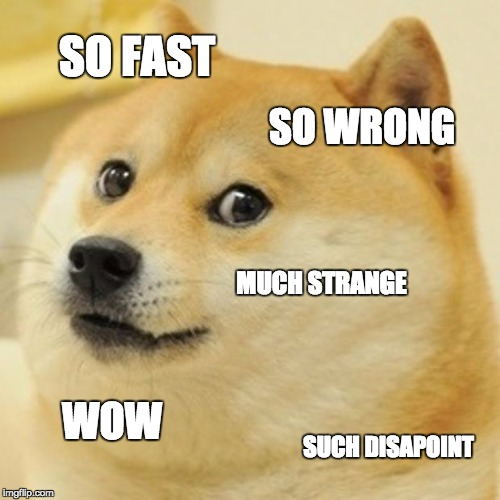
\includegraphics[width=\linewidth]{Z}
%% \caption{Servers are hard to get to produce reliable results.}
%% \end{figure}

In this section, we describe how we will evaluate the practicality of
our discipline.

\subsection{Quantitative Evaluation}

Our first evaluation is a quantitative analysis of running our tool on
an existing repostory. In doing so we hope to answer:

{\bf RQ1.} Does our tool detect SemVer violations?

We know from our proof sketches in section \ref{sec:cvt} that if a
library interface is fully specified, we can accurately detect SemVer
violations. This statement is subject to multiple confounding
factors, including whether tests are expressive enough to detect
violations and whether tests are too strict, which would result in an
over-approximation of the interface.

The first confounding factor can easily be related to the problem of
test coverage. Tests which are too specific may not fully cover all
features of a program. It is therefore reasonable to ask if an
incomplete specification still can report meaningful errors. We have
decided to test our tool on an existing library,
Mocha~\cite{mocha}. Mocha, a test framework, is an ideal tool to test
because it has many versions and is well tested. Mocha contains two
interesting test targets: {\tt test-all}, which runs all tests, and
{\tt test-jsapi}, which tests an internal interface. These tests are
not designed to follow our discipline, but if we assume that they
are, then if we are able to find any violations, we have evidence
that a test suite can be used to define an interface. We run our {\tt
  detect} tool on each release in the library and collect the
Breaking Change and Added Feature violations for each release. For
each version, we report the number violated tests. A test may be
duplicated in the results if it appears is in multiple versions but
this may emphasize the importance of the test, since it survived for
multiple releases.

The second confounding factor is that too many violations may be
reported, which reduces the practicality of our tool. This
confounding factor is also the most controversial. Many developers
have claimed that adhering to SemVer, given their internal definition
of an interface, would force them to bump the major version on every
update~\cite{backbone-2888,exoplayer-1382,crawford-not-semver}. This
problem would be even more pronounced if an interface was clearly
specified using tests and SemVer compliance was checked with a strict
and uncompromising tool. To address this factor, we have created a
simulated version history of Mocha using our approach. This version
history is evidence that following our approach would not be an undue
burden on library authors. It is also a worst-case scenario, where
developers did not expect their tests to be used to describe a public
interface and were not warned about violations before releasing.

\marktodo{this whole paragraph needs work} \-Lastly, we did some background analysis on the framework to better
understand the composition of the library. To do this, we compared the
total number of unique test violations to the total number of unique
tests. This enables us to detect the density of the violations in the
library. This density is interesting when making conclusions about
the two confounding factors, and will help us better determine
whether the findings from this library apply to other libraries.

\subsection{User Study Evaluation}
Our second evaluation is a user study of the efficacy of our
approach. We attempt to answer: 

{\bf RQ2.} Without any assumptions about the test suite, does our tool
detect SemVer violations?

{\bf RQ3.} How difficult is it to adopt our discipline of writing API
tests?

To answer {\bf RQ2}, we manually inspected the {\em possible} 
violations reported by our tool in order to determine whether any of
them represent true violations. In particular, we ask whether the test
failure was due to an illegal change in the interface (in which case
the failure is a true violation), due to non-adherence to our
discipline, or for some other reason.

While reviewing the violations for {\bf RQ2}, we refactored failing
tests to adhere to our discipline whenever possible. To answer {\bf
  RQ3}, we recorded the time required for the refactoring. We also
looked for any inherent limitations of our approach that may make
adherence more difficult.

This study was conducted by the authors, who had no prior knowledge of
the internals of Mocha. Lacking ground truth for what the ``true''
interface is, we consulted the Mocha documentation, source code and
comments, and version history to make the best determination
possible. Whenever multiple interpretations were possible, we gave
Mocha developers the benefit of the doubt, choosing the interpretation
that would minimize SemVer violations.

